%%
%% This is file `sample-acmtog.tex',
%% generated with the docstrip utility.
%%
%% The original source files were:
%%
%% samples.dtx  (with options: `acmtog')
%% 
%% IMPORTANT NOTICE:
%% 
%% For the copyright see the source file.
%% 
%% Any modified versions of this file must be renamed
%% with new filenames distinct from sample-acmtog.tex.
%% 
%% For distribution of the original source see the terms
%% for copying and modification in the file samples.dtx.
%% 
%% This generated file may be distributed as long as the
%% original source files, as listed above, are part of the
%% same distribution. (The sources need not necessarily be
%% in the same archive or directory.)
%%
%%
%% Commands for TeXCount
%TC:macro \cite [option:text,text]
%TC:macro \citep [option:text,text]
%TC:macro \citet [option:text,text]
%TC:envir table 0 1
%TC:envir table* 0 1
%TC:envir tabular [ignore] word
%TC:envir displaymath 0 word
%TC:envir math 0 word
%TC:envir comment 0 0
%%
%%
%% The first command in your LaTeX source must be the \documentclass command.
\documentclass[acmtog]{acmart}
\usepackage{float}

%%
%% \BibTeX command to typeset BibTeX logo in the docs
\AtBeginDocument{%
  \providecommand\BibTeX{{%
    \normalfont B\kern-0.5em{\scshape i\kern-0.25em b}\kern-0.8em\TeX}}}

%% Rights management information.  This information is sent to you
%% when you complete the rights form.  These commands have SAMPLE
%% values in them; it is your responsibility as an author to replace
%% the commands and values with those provided to you when you
%% complete the rights form.
\setcopyright{acmcopyright}
\copyrightyear{2018}
\acmYear{2018}
\acmDOI{XXXXXXX.XXXXXXX}


%%
%% These commands are for a JOURNAL article.
\acmJournal{TOG}
\acmVolume{37}
\acmNumber{4}
\acmArticle{111}
\acmMonth{8}

%%
%% Submission ID.
%% Use this when submitting an article to a sponsored event. You'll
%% receive a unique submission ID from the organizers
%% of the event, and this ID should be used as the parameter to this command.
%%\acmSubmissionID{123-A56-BU3}

%%
%% The majority of ACM publications use numbered citations and
%% references.  The command \citestyle{authoryear} switches to the
%% "author year" style.
%%
%% If you are preparing content for an event
%% sponsored by ACM SIGGRAPH, you must use the "author year" style of
%% citations and references.
\citestyle{acmauthoryear}

%%
%% end of the preamble, start of the body of the document source.
\begin{document}

%%
%% The "title" command has an optional parameter,
%% allowing the author to define a "short title" to be used in page headers.
\title{Spatiotemporal human movement in indoor workspaces: A privacy preserving analysis}

%%
%% The "author" command and its associated commands are used to define
%% the authors and their affiliations.
%% Of note is the shared affiliation of the first two authors, and the
%% "authornote" and "authornotemark" commands
%% used to denote shared contribution to the research.
\author{Ben Trovato}
\authornote{Both authors contributed equally to this research.}
\email{trovato@corporation.com}
\orcid{1234-5678-9012}
\author{G.K.M. Tobin}
\authornotemark[1]
\email{webmaster@marysville-ohio.com}
\affiliation{%
  \institution{Institute for Clarity in Documentation}
  \streetaddress{P.O. Box 1212}
  \city{Dublin}
  \state{Ohio}
  \country{USA}
  \postcode{43017-6221}
}

\author{Lars Th{\o}rv{\"a}ld}
\affiliation{%
  \institution{The Th{\o}rv{\"a}ld Group}
  \streetaddress{1 Th{\o}rv{\"a}ld Circle}
  \city{Hekla}
  \country{Iceland}}
\email{larst@affiliation.org}

\author{Valerie B\'eranger}
\affiliation{%
  \institution{Inria Paris-Rocquencourt}
  \city{Rocquencourt}
  \country{France}
}

\author{Aparna Patel}
\affiliation{%
 \institution{Rajiv Gandhi University}
 \streetaddress{Rono-Hills}
 \city{Doimukh}
 \state{Arunachal Pradesh}
 \country{India}}

\author{Huifen Chan}
\affiliation{%
  \institution{Tsinghua University}
  \streetaddress{30 Shuangqing Rd}
  \city{Haidian Qu}
  \state{Beijing Shi}
  \country{China}}

\author{Charles Palmer}
\affiliation{%
  \institution{Palmer Research Laboratories}
  \streetaddress{8600 Datapoint Drive}
  \city{San Antonio}
  \state{Texas}
  \country{USA}
  \postcode{78229}}
\email{cpalmer@prl.com}

\author{John Smith}
\affiliation{%
  \institution{The Th{\o}rv{\"a}ld Group}
  \streetaddress{1 Th{\o}rv{\"a}ld Circle}
  \city{Hekla}
  \country{Iceland}}
\email{jsmith@affiliation.org}

\author{Julius P. Kumquat}
\affiliation{%
  \institution{The Kumquat Consortium}
  \city{New York}
  \country{USA}}
\email{jpkumquat@consortium.net}

%%
%% By default, the full list of authors will be used in the page
%% headers. Often, this list is too long, and will overlap
%% other information printed in the page headers. This command allows
%% the author to define a more concise list
%% of authors' names for this purpose.
\renewcommand{\shortauthors}{Trovato and Tobin, et al.}

%%
%% The abstract is a short summary of the work to be presented in the
%% article.
\begin{abstract}
  A clear and well-documented \LaTeX\ document is presented as an
  article formatted for publication by ACM in a conference proceedings
  or journal publication. Based on the ``acmart'' document class, this
  article presents and explains many of the common variations, as well
  as many of the formatting elements an author may use in the
  preparation of the documentation of their work.
\end{abstract}

%%
%% The code below is generated by the tool at http://dl.acm.org/ccs.cfm.
%% Please copy and paste the code instead of the example below.
%%
\begin{CCSXML}
<ccs2012>
 <concept>
  <concept_id>10010520.10010553.10010562</concept_id>
  <concept_desc>Computer systems organization~Embedded systems</concept_desc>
  <concept_significance>500</concept_significance>
 </concept>
 <concept>
  <concept_id>10010520.10010575.10010755</concept_id>
  <concept_desc>Computer systems organization~Redundancy</concept_desc>
  <concept_significance>300</concept_significance>
 </concept>
 <concept>
  <concept_id>10010520.10010553.10010554</concept_id>
  <concept_desc>Computer systems organization~Robotics</concept_desc>
  <concept_significance>100</concept_significance>
 </concept>
 <concept>
  <concept_id>10003033.10003083.10003095</concept_id>
  <concept_desc>Networks~Network reliability</concept_desc>
  <concept_significance>100</concept_significance>
 </concept>
</ccs2012>
\end{CCSXML}

\ccsdesc[500]{Computer systems organization~Embedded systems}
\ccsdesc[300]{Computer systems organization~Redundancy}
\ccsdesc{Computer systems organization~Robotics}
\ccsdesc[100]{Networks~Network reliability}

%%
%% Keywords. The author(s) should pick words that accurately describe
%% the work being presented. Separate the keywords with commas.
\keywords{datasets, neural networks, gaze detection, text tagging}


%%
%% This command processes the author and affiliation and title
%% information and builds the first part of the formatted document.
\maketitle

\section{Introduction}
Reopening workplace spaces will inevitably increase contact, interaction, group gathering, and close contacts making it harder to maintain social distancing, moreover, rely on social distance for safety. This, in turn, may raise the risk of transmission inside the workplace. Changes in office layout and increased air ventilation can be useful, but the increase in exposure due to increased person-to-person contact cannot be ignored. According to the World Health Organisation (WHO), the virus that is responsible for human-human transmission may stay viable after aerosolisation in the indoor environment. As a result, while returning to the office spaces, the impacts of human mobility inside the workspace and its impact on the workplace's ability to pose minimal risk must be extensively explored.



This research seeks to model human mobility inside four distinct types of workspaces (a chemistry lab on a university campus, an IT office, a hospital ward, and a factory) while accounting for spatial density, occupancy schedules, and numerous indoor activities. Understanding the mobility of employees at a workplace will enable us to understand their behaviour and identify the day-to-day tasks they undertake as an element of work. Apart from conventional mitigation strategies such as physical distancing, improved ventilation, face masks, and personal hygiene, this will provide methods for establishing coping mechanisms to prevent exposure risk rather than treating such instances as outliers. Because this study aims to forecast human mobility inside a facility, it can be combined with various air quality index measurements to forecast transmission risk, providing numerical clarity on how crowded a workspace or point of interest within the workspace can be while still posing minimal transmission risk. Previous research in this area has focused on either understanding occupant behaviour or exploring the effect of human activities on airflow patterns in the instance of a single person model in a controlled setting. There is a lot of research on using Wi-Fi access point data to model human mobility inside buildings \cite{qian2016decimeter}, \cite{meneses2012large} but not much work has been done in a detailed manner for specific spaces, such as a single lab or a workspace. In terms of studying the influence of human movement on indoor airflow patterns, most experiments have been carried out in a plotted methodology where the trajectory of the person was already planned \cite{mahaki2021comparing}, \cite{wu2022transient}. But the challenge is to correlate the behaviour of occupants with the airflow patterns in the space while preserving the privacy of the occupants. We perform privacy-preserving analysis in the wild, where the trajectory of participants and the air-quality index are the only data points collected. The context or the labels (such as the schedule of meetings) of events occurring in the workspace (such as the roster of employees working from the office) during the monitoring period are not known. This introduces a lot of apprehension in the process of modelling and generalising movement behaviour, which is dealt with by devising a set of uncertainty-aware rules to interpret the trajectories. To the best of our knowledge, this is the first work that studies the movement behaviour of occupants in an indoor office space and interweaves it with the airflow patterns in the presence of airborne disease. We explore the various aspects of indoor human movement throughout time and space by answering the following questions:
\begin{itemize}
    \item Do employees have a habit of visiting similar locations in the workplace?
    \item Do employees use the same routes to get from one location to another within the office?
    \item Is there a difference in the pattern of human movement during the day or between days?
    \item Is there a relationship between human movement and the density of airborne pathogens in different areas indoors?
    \item Are there any hot pockets (preferred stations, printing desk) inside the office space?
    \item Do the hot pockets get congested/crowded at regular intervals?
    \item Do the common footpaths inside the workspace pose a higher risk of transmission at all times?
    \item Do factors like sitting location, interconnecting doors, crowdedness and air quality influence human movement patterns indoors (geometric and non-geometric factors)?
\end{itemize}



Preventing the risk of infection and close contact is now part of workplace safety, posing a new challenge for sustaining workplace quality, promoting a sense of fulfilment and satisfaction, and enhancing productivity. A safer workplace will not only encourage employees to return in comfort but will also boost their performance. Because our work considers multiple kinds of workplaces, developing context-based workplace safety guidelines will serve a broader community. Therefore, the main contributions of this work are:
\begin{itemize}
    \item Indoor human movement study, we present an analysis of the spatiotemporal trajectories of employees inside the workspace.
    \item Event-based human-environment interaction approximation, we perform an event-based correlation between the human mobility trends and the airflow patterns inside the workspace.
    \item Spatial Context-based safety guidelines, we demonstrate practical implications of the relations between human movement and airflow patterns across workspaces.
\end{itemize}
The rest of this paper is organised as follows, we begin by reviewing the recent research work in this domain and identify the gaps in the literature. Then we introduce the utilised terminologies and describe the collected dataset after which we explain the methodology, elaborate on the analysis, and the results and discuss the relations between human movement and airflow patterns across workspaces before summing it up in the conclusion.


%%%%%%%%%%%%%%%%%%%%%%%%%%%%%%%%%%%%%%%%%%%%%%%%%%%%%%%%%%%%%%%%%%%%%%%%%%%%%%%%%%%%%%%%%%%%%%


\section{Related work}
With the outbreak of the pandemic and the struggle to reinstate office spaces, a lot of research has been done to reduce the risk of exposure in various types of indoor environments. Although the majority of developments in this field can be classified into three categories: safer indoor navigation, contact tracing and avoidance, and building occupancy simulation, there has also been some research to investigate the effects of human movement on air particles in an indoor space.

\subsection{Safer indoor traversal}

Costa and Ge et al. introduced a graph-based indoor-outdoor path technique that examines both the exterior graph of buildings and streets and the interior graph of the entrances and exits within each building to construct a unified, context-aware path \cite{costa2019caprio}. Jensen and Nielsen et al. created an algorithm that can traverse both indoor and outdoor spaces and yield the true shortest path between two arbitrary points \cite{jensen2016outdoor}. Salgado \& Cheema et al. used the Global Category Nearest Neighbour approximation method to conduct category aware multi-criteria route planning, which provides an ideal route between two indoor places by taking into consideration the inside, the outdoors, and semi-indoors \cite{salgado2018efficient}.

\subsection{Contact tracing and contact avoidance}

Trivedi et al. developed WiFiTrace, a network-centric approach to contact tracing that relies on passive WiFi sensing with no client-side involvement. They used WiFi network logs collected by enterprise networks for performance and security monitoring to reconstruct device trajectories for contact tracing \cite{trivedi2021wifitrace}. YYue et al. propose a neural network model termed Spatio-Temporal Episodic Memory for COVID-19 (STEMCOVID) that uses contact tracking data to detect infectious asymptotic instances. The model encodes a collective Spatio-temporal episodic memory of individuals and contains an effective parallel search mechanism based on the fusion Adaptive Resonance Theory (ART) \cite{hu2020silent}. Avoiding contact may also be accomplished by minimising congestion, which can be achieved with the help of congestion forecasting, a field that has experienced tremendous growth during the pandemic. ABy utilising the building floor plan and modelling human trajectory as a Gaussian distribution, Anastasiou and Costa et al created a platform for indoor congestion generation to facilitate congestion forecasting in indoor settings \cite{anastasiou2021epicgen}. Using Wi-Fi access points, Abrishami and Kumar constructed a model for estimating foot traffic for retailers inside a shopping mall \cite{abrishami2018using}. Islam and Gandhi et al. offer a collaborative filtering strategy based on tensor factorization that uses granular real-time foot traffic data to determine foot traffic for a point of interest \cite{islam2021spatiotemporal}. Using game theory, Xie and Luan et al devised a crowdsourcing-based indoor navigation model that encourages users to use navigation services. \cite{xie2021game}.

% Please add the following required packages to your document preamble:
% \usepackage{graphicx}
% \usepackage[table,xcdraw]{xcolor}
% If you use beamer only pass "xcolor=table" option, i.e. \documentclass[xcolor=table]{beamer}
\begin{table*}[!h]
\centering
\caption{Review of recent works investigating the impact of human movement on air particles in indoor spaces}
\label{tab:my-table}
\resizebox{\textwidth}{!}{%
\begin{tabular}{llllll}
\hline
{\color[HTML]{0E101A} Title} & {\color[HTML]{0E101A} Purpose} & {\color[HTML]{0E101A} Sensors used} & {\color[HTML]{0E101A} Size of dataset} & {\color[HTML]{0E101A} Models human mobility} & {\color[HTML]{0E101A} \begin{tabular}[c]{@{}l@{}}Conducted in the\\  presence of an \\ airborne disease\end{tabular}} \\ \hline
{\color[HTML]{0E101A} \begin{tabular}[c]{@{}l@{}}Occupant behaviour and\\  indoor particulate\\  concentrations in\\  daycare centres \cite{um2022occupant}\end{tabular}} & {\color[HTML]{0E101A} \begin{tabular}[c]{@{}l@{}}To analyse the effect \\ of human activity and\\  human-building \\ interaction on indoor air quality.\end{tabular}} & {\color[HTML]{0E101A} \begin{tabular}[c]{@{}l@{}}Optical particle counters, \\ real-time CO2 measurement\\ and window state data  loggers\end{tabular}} & {\color[HTML]{0E101A} Approximately 780hrs} & {\color[HTML]{0E101A} \begin{tabular}[c]{@{}l@{}}No, present a \\ discussion based \\ on scheduled activities\end{tabular}} & {\color[HTML]{0E101A} No} \\ \hline
{\color[HTML]{0E101A} \begin{tabular}[c]{@{}l@{}}Transient and continuous\\  effects of indoor human \\ movement on nanoparticle\\  concentrations in a sitting\\  person's breathing zone \cite{wu2022transient}\end{tabular}} & {\color[HTML]{0E101A} \begin{tabular}[c]{@{}l@{}}To sample the nanoparticle\\  concentration in the \\ breathing zone of a \\ sitting thermal\\  breathing manikin (STBM).\end{tabular}} & {\color[HTML]{0E101A} \begin{tabular}[c]{@{}l@{}}Sitting thermal breathing \\ manikin (STBM), Aerosol \\ generator and a medical ventilator\end{tabular}} & {\color[HTML]{0E101A} \begin{tabular}[c]{@{}l@{}}NA, controlled\\ singular experiment\end{tabular}} & {\color[HTML]{0E101A} No} & {\color[HTML]{0E101A} No} \\ \hline
{\color[HTML]{0E101A} \begin{tabular}[c]{@{}l@{}}Comparing objects for\\  human movement \\ simulation regarding\\  its air flow disturbance\\  at local exhaust ventilation \cite{mahaki2021comparing}\end{tabular}} & {\color[HTML]{0E101A} \begin{tabular}[c]{@{}l@{}}To study the disturbances\\  due to the movements \\ of a human-sized plate,\\  cylinder and detailed\\  manikin near a ventilation hood.\end{tabular}} & {\color[HTML]{0E101A} \begin{tabular}[c]{@{}l@{}}3-D sonic anemometer for\\  velocity measurements\end{tabular}} & {\color[HTML]{0E101A} \begin{tabular}[c]{@{}l@{}}NA, controlled\\ singular experiment\end{tabular}} & {\color[HTML]{0E101A} No} & {\color[HTML]{0E101A} No} \\ \hline
{\color[HTML]{0E101A} \textbf{\begin{tabular}[c]{@{}l@{}}Spatiotemporal human\\  movement in indoor\\  workspaces: A privacy\\  preserving analysis\end{tabular}}} & {\color[HTML]{0E101A} \textbf{\begin{tabular}[c]{@{}l@{}}To model the spatiotemporal \\ movement of employees \\ inside workspaces and \\ analyse their effect on\\  indoor airflow\end{tabular}}} & {\color[HTML]{0E101A} \textbf{\begin{tabular}[c]{@{}l@{}}Bluetooth tags for \\ RSSI signals and surveys\end{tabular}}} & {\color[HTML]{0E101A} \textbf{\begin{tabular}[c]{@{}l@{}}8 days for Bluetooth \\ tags, one month of survey data\end{tabular}}} & {\color[HTML]{0E101A} \textbf{Yes}} & {\color[HTML]{0E101A} \textbf{Yes}} \\ \hline
\end{tabular}%
}
\end{table*}
\subsection{Occupancy risk estimation}
Sydora et al. provide a systematic simulation-based technique for calculating the infection risk for inhabitants of a building under various scenarios of building utilisation, as well as a virus transmission model that evaluates the possible infection transmission risk based on occupant behaviour \cite{sydora2022building}. Ciunkiewicz et al. devised an agent-based simulation (ABS) framework for localised settings that is highly configurable. This ABS enables extensive control over COVID-19's fast-growing epidemiological features, as well as information on risk and the impacts of both pharmaceutical and non-pharmacological interventions \cite{ciunkiewicz2022agent}. The findings of simulations can help facility administrators make better decisions and can also be utilised as inputs for a decision support system. 

\subsection{Studying indoor occupant behaviour}
Lee et al. investigate the effects of spatial and temporal restrictions in a facility, which might limit occupants' capacity to physically remove themselves, by conducting a survey to see if and how such constraints affect occupants' physical distancing behaviours in K–12 educational facilities \cite{lee2022understanding}. Jayjarah et al. developed a methodology for predicting the Likelihood of Future Non-Conformance (LFNC), which is based on the hypothesis that the likelihood of future deviations in movement behaviour is positively correlated to the intensity of trajectory deviations observed in the user's recent past and that the likelihood of future deviations increases if the user's strong-ties have also recently exhibited such non-conformant movement behaviour using longitudinal indoor location data from a university campus \cite{jayarajah2018predicting}. Chen et al. present a large-scale systematic analysis in the context of urban revisitation and re-check-in, demonstrating people's periodic behaviours and regularities by leveraging a localisation dataset to model urban revisitation and identifying features concerning POI visitation patterns, POI background information, user visitation patterns, user preference, and users \cite{chen2020will}.



\subsection{Investigating the impact of human movement on air particles in indoor spaces}
 Indoor airflow patterns are known to be influenced by human activities and their aerodynamic impact depends on factors like speed, distance as well as position in space. Pollutants are released into indoor air by people, occupant activities, building materials, and even outside air. Using optical particle counters (OPS) for particulate concentration monitoring and resuspending source strengths of particles with characteristics of human-building interactions, Um et al. investigated the effects of occupant behaviour on indoor particle concentrations in daycare centres in four daycare centres in South Korea and found that vacuuming should be avoided while the daycare facility is occupoed by children. The results also indicated that indoor air quality can be severely degraded by opening windows without considering the level of outdoor particle concentration \cite{um2022occupant}.  Wu et al. performed a series of experiments to sample the nanoparticle concentration in the breathing zone of a sitting thermal breathing manikin (STBM) in order to investigate transient variability in nanoparticle concentration. They discovered that continuous exposure to a sitting person can result in a 2.88 (1.24) percent increase in nanoparticle concentration \cite{wu2022transient}. Mahaki et al. used a human-sized plate, cylinder, and detailed manikin to study the effects of human movement on airflow patterns around local ventilation hoods both experimentally and numerically, with the movements consisting of back-and-forth movements near an exhaust hood using a 3-D sonic anemometer to measure air velocity in front of the hood opening. The results revealed that the turbulence created by the object's motions contained distinct air velocity peaks in the near field of the exhaust hood, both supporting and inhibiting the suction flow \cite{mahaki2021comparing}.



Although some research has been done on modelling human movement for indoor environments and analysing the impact of human movement on airflow patterns inside a space, it has all been conducted in a controlled environment and thus does not take into account the spatiotemporal elements that may limit the occupant's ability to maintain a safe distance at all times or influence occupant behaviour or the day-to-day workplace habits, which may, in turn, drive the airflow pattern. Most studies consider the overall picture of the building, but what happens inside during working hours or scheduled activities, and its impact on controlling or lowering the risk of infection, are yet unknown. There are broad rules for personal hygiene and social distance, but in a space that is used by a variety of individuals throughout the day, as well as visitors and passers-by, the assumption that "if everyone does their bit, we'll all be safe" may not be sufficient.
Therefore the following gaps exist in the literature:
\begin{itemize}
    \item Lack of understanding about the spatiotemporal human movement inside different kinds of workspaces.
    \item Lack of a framework that correlates the indoor airflow pattern of a workspace with their respective human movement trends.
    \item Lack of understanding of the practical implications of the relations between human movement and airflow patterns across workspaces.
\end{itemize}


%%%%%%%%%%%%%%%%%%%%%%%%%%%%%%%%%%%%%%%%%%%%%%%%%%%%%%%%%%%%%%%%%%%%%%%%%%%%%%%%%%%%%%%%%%%%%%


\section{Data Collection}
We conducted the study at four sites, including a chemistry wet lab at RMIT University, an IT office, a Covid-19 ward inside a hospital and a factory, the and the data collection process was approved by the Human Research Ethics Committee at our University. The duration of data collection was different for different sites and the data was collected in two forms, participant trajectories using BLE tags and a survey.

\subsection{Participants}
Participants were recruited for each site. Employees/students at each site were briefed about the study as well as the data collection process. Those who volunteered to participate in the study were asked to fill and sign consent forms which were collected and stored in a locked box to preserve the privacy of the participants. Details about the consent form..... After they returned the signed consent forms, they were asked to take a Bluetooth tag to carry with them throughout the study. The participants were asked to carry the same tag for the whole period of the study. No participant information associated with the tag was obtained. The participants were also asked to complete a 15-question survey twice every day. The participants had to use their email address to register for the daily survey reminders but their email address was not correlated with any other information and was solely used to send survey reminders. No personal information was recorded in the survey either.

\subsection{Collected Data}
\subsubsection{Movement Data}
To record the movement of participants in their workspaces, they were asked to carry Kontakt Asset Tag-2(s) in their pockets for the period of the study. The participants were asked to carry the same tag for the entire duration of the study but the details about the participant associated with the tag were not recorded. Kontakt Asset Tag-2 are Bluetooth based tags that are equipped with a 3DH motion sensor and are capable of over-the-air communication using Bluetooth over a range of up to 50m. The BLE signals broadcasted by these tags are detected and collected by gateways. Kontakt portal lights that are plug and play BLE gateways were used to receive these signals. The Asset Tag-2 is also equipped with an IR receiver which when combined with the portal light can provide room-level location accuracy. The portal lights can leverage the already existing Wi-Fi network and also have a Bluetooth range of 50m. 
The Asset Tag-2 are transmitters and have a unique identifying code which they transmit using Bluetooth Low Energy technology to the nearby receivers which are the Kontakt portal lights in this case. The transmitted unique Asset Tag identifier (i.e. tracking id) can be used to detect the presence and movement of a person carrying a specific beacon. A gateway device passively scans for BLE card beacons in its surrounding range. Upon detection of beacons, the gateway continuously collects beacon data including their unique identifiers, can start and end timestamps, and RSSI. The gateway uses RSSI to determine the proximity of the beacons with the gateway. Gateways send the collected beacon data to the cloud storage server approximately every 5 seconds.
\begin{figure}[h]
  \centering
  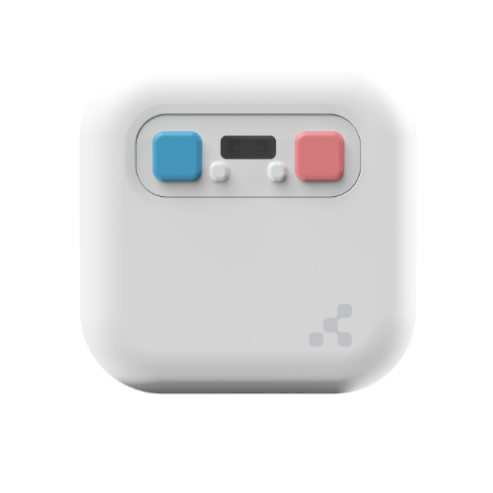
\includegraphics[width=3cm,height=3cm,keepaspectratio]{Asset-Tag-493x0-c-default}
  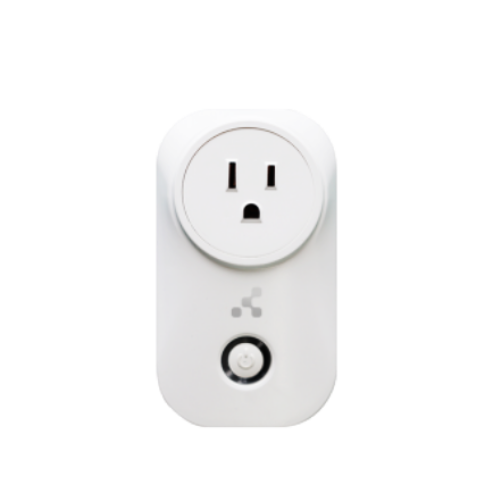
\includegraphics[width=4cm,height=4cm,keepaspectratio]{Group-15446-493x0-c-default}
  \caption{Kontakt Asset Tag-2 and Gateway}
  \end{figure}
\subsubsection{Survey Data}
The participants were asked to fill a 15-question survey twice every day for the duration of the study (if they were working from the office). This survey was intended to capture ground truth about the movement habits of the participants inside the workplace. It included questions about the seating location of the participant, their most used footpath inside the space, their interactions with co-workers, whether or not they interacted with people around them, their trips away from the workstation, the noise and their concentration levels. It also contained a question on whether or not they were wearing masks. The participants were also encouraged to mention their Asset tag ID in the survey response to enable comparison with movement data and the survey responses. To ensure participant privacy, no personal details were collected by the survey and hence the Asset tag ID could not be used to retrace the participant.

\subsection{Procedure}
Before the data collection, all Asset tags were synchronised and configured to a level 2 (available values were 1-5) of signal transmission that emits up to a range of 10m as it gave the best location accuracy for our experimental setup. The advertising rate was set to 100ms. The gateways were used with the default configurations and a designated Wi-Fi network was laid out for them. 
\begin{figure}[h]
  \centering
  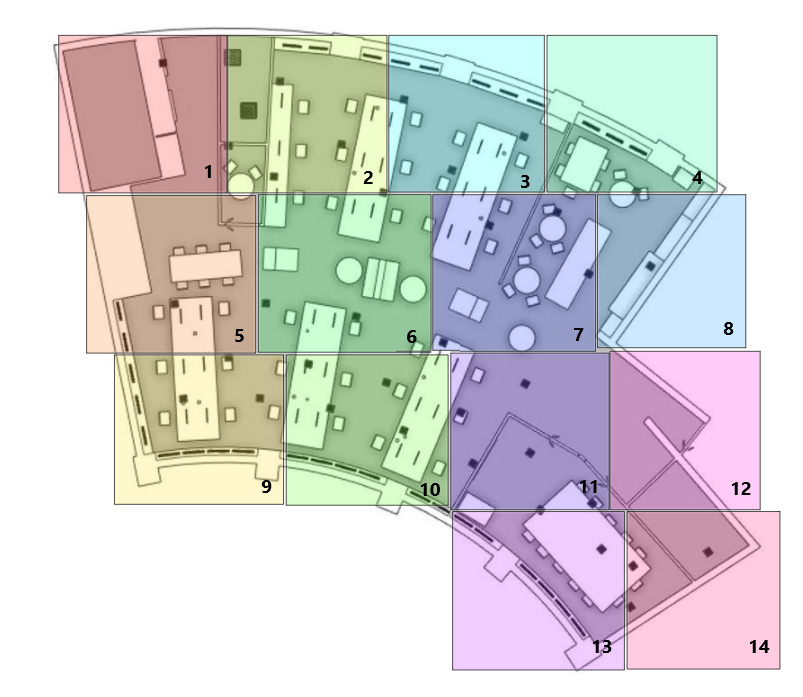
\includegraphics[width=4cm,height=4cm,keepaspectratio]{grids.png}
  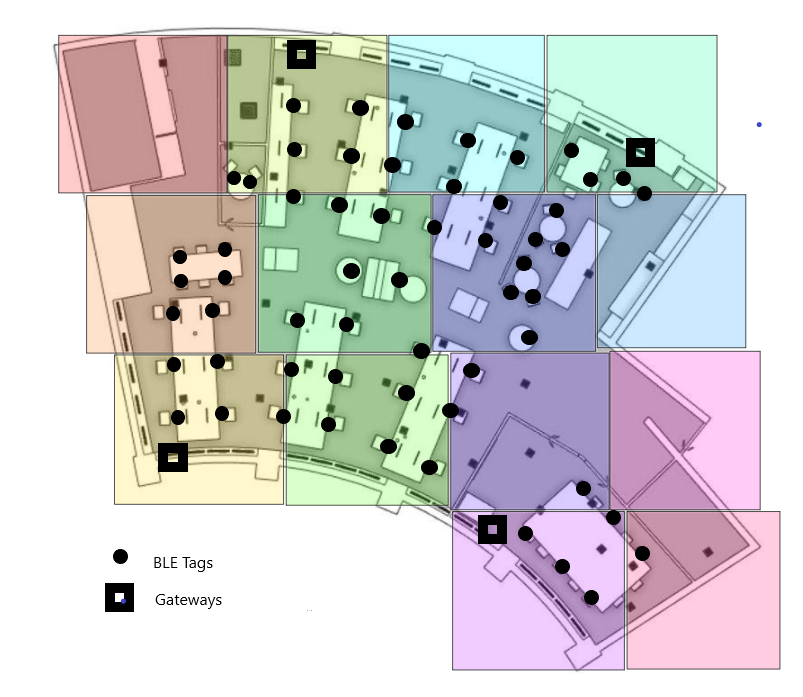
\includegraphics[width=4cm,height=4cm,keepaspectratio]{sensors_grids.png}
  \caption{Workspace divided into 14 grids (left) and the stationary tags deployed for fingerprinting along with the gateways (right)}
  \label{Memkogrids}
  \end{figure}
For the purpose of the experiment, the office space was divided into 14 equal-sized grids as shown in Figure-\ref{Memkogrids} (left). Workstations, meeting and conference rooms, kitchen space, and the printing station are all covered by the grids. We then carried out a fingerprinting experiment that was later utilised to train the localisation model. To perform the fingerprinting, we placed 4-5 Asset Tags in each grid, for two days, to mimic the presence of employees in those grids.  There were a total of 65 stationary tags deployed inside the office space along with four gateways as shown in Figure-\ref{Memkogrids} (right). We collected 2000 continuous data points per tag and trained the localisation model as follows. We selected a duration of 20 seconds (the 30s was also used but the accuracy was better with 20s) to segment the continuous data points proportionally and then extracted statistical features like the minimum, maximum, mean, median, variance, first quartile and the third quartile. We also had the timestamps and the occupancy labels (grid ID) of the stationary tags which we segmented using the same duration. This gave us a dataset imitating employees in the workspace with RSSI features and labelled occupancy values which we used for predicting the locations of employees. We trained three classification models, namely Support Vector Machine (SVM), Logistic Regression and K-nearest neighbour (n=5) and evaluated their performance on the test set (20 per cent of the data was used for testing), out of which K nearest neighbour performed the best reporting accuracy of 70 per cent. The accuracy of prediction was calculated by taking the ratio of correctly predicted instances to the total number of instances evaluated. We admit that the stationary tags may not mimic the movement of employees inside the workspace but since it was not feasible to conduct a fingerprinting experiment by moving around the office during working hours, we placed multiple tags in each grid to generate a sense of the various locations the employees may be present at. 
\begin{itemize}
    \item After establishing the localisation model, the participants were asked to take an Asset Tag each, we had 13 participants for a period of 6 days and collected 12,000 trajectories per participant. 
    \item The survey was sent on all working days at 11:00 AM and 16:00 PM, we received an average of 8 daily responses making it a total of 173 responses. Approximately 40 per cent of the employees working from the office volunteered to participate in the survey. 
    \item At the end of the data collection period, the participants were asked to return the Asset Tags in the designated box. 
\end{itemize}

%%%%%%%%%%%%%%%%%%%%%%%%%%%%%%%%%%%%%%%%%%%%%%%%%%%%%%%%%%%%%%%%%%%%%%%%%%%%%%%%%%%%%%%%%%%%%%


\section{Data preprocessing}
The process of data cleaning was carried out in two steps, first cleaning instances in the raw RSSI data where the tag could not be detected by all four gateways and hence the RSSI values for some gateways is 0. This could be due to a technical issue in the network or due to the tag being out o freach for one or more gateways. In this case, the best possible values were used. The second step involves cleaning the predicted employee trajectories, because the prediction model was trained only for two days and on stationary, it predicted the employee hopping over several grids in a very short duration.  
After using the localisation model to predict the locations of the employees, the resulting dataset comprised of timestamp, Asset Tag ID and the grid-ID. Using some dataframe manipulation functions from the pandas library, features like previous grid-ID, next grid-ID, status of grid change and the time spent in the grid were computed. On analysing the trajectories of employees, it was observed that the dataset contained significant amount of noise. Therefore, the following rules were used to clean the data.
  
\begin{itemize}
    \item There were a lot of instances where the users' location was being picked up as a nearby grid, just for one instance, since these hops were less than a second in duration and were redundant throughout the data, all such instances were labled as the user's seating location using as follows:
    \item In some instances the employee was seated on the border of two grids, causing the model to predict the presence of the employee in the second grid quite often. This was a pattern across all employee trajectories where there was atleast one nearby grid which had been predicted as the location and the movement to and from that grid was random and redundant across all days as well as every hour of the day. Therefore, for each employee, this psedo-location was identified and labelled as their seating location.
    \item Noise was observed not only for the instances around the seating location but also when the user was not present at their seating location. Therefore, if the employee's trajectory reflected frequent hops between two nearby grids, they were merged into the grid the user was initially at, or spent more time at.
    
\end{itemize}


We admit that we do not have any ground truth behind these rules used for noise removal but they were carefully devised by taking into consideration the presence of common patterns across all days or each hour of the day and sometimes for every user.



%%%%%%%%%%%%%%%%%%%%%%%%%%%%%%%%%%%%%%%%%%%%%%%%%%%%%%%%%%%%%%%%%%%%%%%%%%%%%%%%%%%%%%%%%%%%%%

\section{Methodology}

Modifying the template --- including but not limited to: adjusting
margins, typeface sizes, line spacing, paragraph and list definitions,
and the use of the \verb|\vspace| command to manually adjust the
vertical spacing between elements of your work --- is not allowed.

\subsection{Terminologies}
\subsubsection{Human Movement}
The term human movement in context of this study refers to the movement of employees across grids for the sake of this research, taking into account the presence of numerous persons in a single grid as well as one or more employees travelling across various grids at the same time. This research does not take into consideration an employee's mobility inside a grid.

\subsubsection{Seating location} The seating locaion for each employee for this analysis has been taken as the grid where the employee spends maximum time, on most days, the value of which is the ID of that grid.

\subsubsection{Trajectory} An instance of an employee present in the workspace where their location can be estimated within the workspace is considered as its trajectory for this study. 

\subsubsection{Nearby grids} The grids located close or around a grid, were classified as nearby grids. Each grid has at least one nearby grid, the list of nearby grids for every grid is mentioned in Table-2. 




\section{Analysis of workspace behaviour}



\section{Results and Discussion}



\section{Authors and Affiliations}



\section{Rights Information}



\section{CCS Concepts and User-Defined Keywords}

Two elements of the ``acmart'' document class provide powerful
taxonomic tools for you to help readers find your work in an online
search.

The ACM Computing Classification System ---
\url{https://www.acm.org/publications/class-2012} --- is a set of
classifiers and concepts that describe the computing
discipline. Authors can select entries from this classification
system, via \url{https://dl.acm.org/ccs/ccs.cfm}, and generate the
commands to be included in the \LaTeX\ source.

User-defined keywords are a comma-separated list of words and phrases
of the authors' choosing, providing a more flexible way of describing
the research being presented.

CCS concepts and user-defined keywords are required for for all
articles over two pages in length, and are optional for one- and
two-page articles (or abstracts).

\section{Sectioning Commands}

Your work should use standard \LaTeX\ sectioning commands:
\verb|section|, \verb|subsection|, \verb|subsubsection|, and
\verb|paragraph|. They should be numbered; do not remove the numbering
from the commands.

Simulating a sectioning command by setting the first word or words of
a paragraph in boldface or italicized text is {\bfseries not allowed.}

\section{Tables}




%%
%% The acknowledgments section is defined using the "acks" environment
%% (and NOT an unnumbered section). This ensures the proper
%% identification of the section in the article metadata, and the
%% consistent spelling of the heading.
\begin{acks}
To Robert, for the bagels and explaining CMYK and color spaces.
\end{acks}

%%
%% The next two lines define the bibliography style to be used, and
%% the bibliography file.
\bibliographystyle{ACM-Reference-Format}
\bibliography{base}

%%
%% If your work has an appendix, this is the place to put it.
\appendix



\end{document}
\endinput
%%
%% End of file `sample-acmtog.tex'.
